\documentclass[12pt]{article}

\usepackage{fullpage}
\usepackage{graphicx}
\usepackage{amsfonts}
\usepackage{amsmath}
\usepackage{graphics}
\usepackage{multirow}
\usepackage{mdwlist, enumerate}


% christos: these look closer to NSF specs\dots
\setlength{\oddsidemargin}{0.0in}
\setlength{\evensidemargin}{0.0in}
\setlength{\textwidth}{6.5in}
\setlength{\headheight}{0.0in}
\setlength{\topmargin}{0.0in}
% \setlength{\textheight}{9.0in}
\setlength{\textheight}{9in}
\addtolength{\textheight}{-\topmargin}
\addtolength{\textheight}{-\headheight}
\addtolength{\textheight}{-\headsep}
\addtolength{\textheight}{-\footskip}



\begin{document}

\newcommand{\beq}{\begin{equation}}
\newcommand{\eeq}{\end{equation}}
\newcommand{\bit}{\begin{itemize*}}
\newcommand{\eit}{\end{itemize*}}
\newcommand{\goal}[1]{ {\noindent {$\Rightarrow$} \em {#1} } }
\newcommand{\hide}[1]{}
\newcommand{\comment}[1]{ {\footnotesize {#1} } }
\newtheorem{lemma}{Lemma}
\newtheorem{theorem}{Theorem}
\newtheorem{proof}{Proof}
\newtheorem{defn}{Definition}
\newtheorem{algo}{Algorithm}
\newtheorem{observation}{Observation}

\title{Dense Subtensor Mining using SQL}


\author{ {\em Jining Qin} \\
	    Dept. of Statistics \\
	    Carnegie Mellon University\\
	    {\tt jiningq@andrew.cmu.edu}
	 \and
	 {\em Lingxue Zhu} \\
	     Dept. of Statistics \\
	    Carnegie Mellon University\\
	     {\tt lzhu1@andrew.cmu.edu}
        }


\maketitle

\section{Introduction}
   \label{sec:introduction} 
   %!TEX root = progress_report.tex

On the large scale, genuine users' activities on the Internet should be randomly distributed over time and space. There are certain areas and time periods associated with higher activity frequency, yet the transition between different time and space are usually smooth. Fraudulent activities, however, often comes with very high frequency within a certain time period, from a particular range of internet devices. For example, spam ratings on various review websites are usually published within a narrow time period, from a certain set of IP addresses. DDoS attacks often feature an overwhelming amount of packets such as TCP, UDP, and IMCP sent from a set of IP addresses (controlled by the attacker) to another particular set of IP addresses associated with the target site or service. Therefore, identifying dense subtensors in the activity databases would be helpful to detecting fraudulent or malicious activities.

The task of mining dense subtensors, however, is challenging in many aspects. The database could have a handful of dimensions, making brute force search impractical. Depending on particular application, the database could vary from easy to handle with a laptop to impossible for a regular cluster. Whatever method we want to use must be able to scale with the size of the problem. That's why SQL is a good platform for implementing the solution. The activity log databases are naturally relational databases easily described by tables. Also, SQL allows for easy and quick data retrieval and manipulation even on large datasets that don't fit in the computer memory, which frees us up from worrying about low-level problems such as data storage and querying.

In this project, we will be implementing the Dcube(\cite{shin2017d}) algorithm in SQL. We will use this subtensor mining algorithm to identify fraudulent ratings in review databases as well as malicious packets in the DARPA TCP dump database. We will then try to optimize our implementation using the indexing methods covered in this course. We will evaluate our implementation using various unit tests and on labeled data using standard tools such as the ROC curve. 

\section{Survey}
    \label{sec:survey}
    %!TEX root = proposal.tex

Next we list the papers that each member read, along with their summary and critique.

\subsection{Papers read by Jining Qin}
%%%%%%%%%%
%% 1
%%%%%%%%%%

\subsubsection{General suspiciousness metric and CorssSpot algorithm \cite{jiang2015general} }

\paragraph{Problem} The main problem that this paper addresses is to propose a formal set of axioms that regulates the suspiciousness metric of a dense block in multimodal data. A metric is then proposed that satisfies the set of axioms and is fast to compute. Then an algorithm CROSSSPOT is proposed to find dense regions and sort them in suspiciousness order, which works well in their experiments on retweet boosting detection.

\paragraph{Main idea} 
There are many works that aim at identifying dense subtensor in multimodal data, yet there is not yet a disciplined method for rating and ranking each suspected dense block. Formally, each dataset is seen as a $K$-mode tensor $X$ with size $\mathbf{N}$ and mass $C$ (the sum of events in the tensor), and the suspected subtensor is denoted $Y$, with size $\mathbf{n}$ and mass $c$.

The axioms on the suspiciousness metric $f(\mathbf{n}, c, \mathbf{N}, C)$ (which can be reparameterized as $\hat{f}(\mathbf{n}, \rho, \mathbf{N}, p)$, where $\rho$ and $p$ denote the density of the corresponding tensor/subtensor) is as follows:

\begin{enumerate}
\item {\it Density} Other things being equal (size), the subtensor with greater mass is more suspicious.

\item {\it Size} Other things being equal (density), the larger subtensor is more suspicious.

\item {\it Concentration} Other things being equal (mass), the smaller block is more suspicious.

\item {\it Contrast} Other things being equal(size), the block in the sparser background tensor is more suspicious.

\item {\it Mltimodal} A block which contains all possible values within a mode is just as suspicious as if the mode was collapsed into the remaining modes.

\end{enumerate}

Following these axioms, the authors proposed a suspiciousness metric, which is the negative log likelihood of block's mass under an Erdos-Renyi-Poisson model. Given an $n_1 \times n_2 \times \cdots, \times n_k$ block of mass $c$ in $N_1 \times N_2 \times \cdots \times N_K$ data of total mass $C$, the suspiciousness score is 
$$f(\mathbf{n}, c, \mathbf{N}, C) = -\log(Pr(Y_n = c))$$
where $Y_n$ is the sum of entries in the block.

A local search algorithm is then proposed to search for suspicious blocks in the dataset. Given a seed region, we loop through each mode of it. The attribute values of each mode is adjusted by including the values which induce the largest amount of intersections of other (fixed) attribute values up to the point that the suspiciousness score is maximized. Such mode adjustment is made iteratively until the region becomes stable. It can be shown that the algorithm is relatively robust to seed region selection, therefore a random seed region would be adequate. Also, the algorithm is quasilinear in the size of the tensor $N$ and linear in the number of non-zero entries.

\paragraph{Connection to our project} The most important contribution of this paper is that we have a disciplined way to think of suspicious subtensors in terms of its size, mass, and contrast with its background tensor. The proposed suspicious metric and algorithm could both be applied (maybe after slight modification) in our project to identify suspicious dense blocks.

\paragraph{Potential shortcomings} The assumption behind the suspiciousness metric might be a little strong. Data generating process might not always follow an Erdos-Renyi-Poisson model. Therefore there is room for generalization of the metric into more relaxed settings. Also, the proposed algorithm (may) require data to be stored in the main memory, which isn't realistic for larger scale problems. The iterative nature of the algorithm makes it hard to scale or parallelize.


%%%%%%%%%%
%% 2
%%%%%%%%%%
\subsubsection{M-zoom \cite{shin2016m} }

\paragraph{Problem}  This paper proposed an flexible algorithm which finds dense block in tensors that is efficient, with accuracy guarantee, and adjustable for different desnity measures. It scales linearly with all aspects of tensors and achieves enormous speedup based on current methods. It is provably accurate on the lowest density of blocks it finds. It supports multi-block detection, size bounds, and diverse density measures. And it works well on the experiment in detecting edit wars and bot activities in Wikipedia and spotting network attacks.

\paragraph{Main idea} 
The outline of M-zoom algorithm goes as follows. M-Zoom copies the entire relation into the main memory. And then finds $k$ dense blocks one by one from it. After finding each block, the entries in the block is removed to prevent the same block from being detected repeatedly. Note that the final output blocks are the blocks corresponding to the attribute values in the found blocks. Therefore it is possible for an entry to appear in more than one identified blocks. In other words, M-zoom is able to find overlapped blocks.

The single block identification algorithm given the relation goes like this. The block is initialized to be the entire remaining relation. Then attributes are removed one by one until the block is empty. M-zoom always find the attribute value after whose removal the block's density could be maximized. A snapshot of this block is then saved for later use. When all attribute values are removed. M-zoom would scan through the snapshots and return the block with the maximum density in the list.


\paragraph{Connection to our project} The algorithm M-zoom looks ideal for problems that fits in the main memory. It is efficient, provably accurate and flexible to different density measures. It also appears to work well on real world data. It is helpful to consider it or its variant in our project. 

\paragraph{Potential shortcomings} The algorithm requires data to fit in main memeory. Therefore it might be limited in application on large scale problems. Also, the accuracy guarantee, though useful, might not be realistic.


%%%%%%%%%%
%% 3
%%%%%%%%%%
\subsubsection{D-cube \cite{shin2017d}}

\paragraph{Problem} The D-cube algorithm also addresses the problem of identifying high-density blocks in multimodal tensors. In particular, it works under the situation where dataset doesn't fit on the main memory, making I/O expense no longer negligible. It is disk-based and can be run in a distributed manner across multiple machines. It achieves massive speedup, memory efficiency, and provable accruacy guarantee. It works well in the experiment of identifying network attacks in real world dataset. 

\paragraph{Main idea} Given a large-scale realtion not fitting in memory, we want to find $k$ distinct blocks with the highest density in terms of the given density measure. The main outline of the algorithm is very close to that of M-zoom. The $k$ blocks are identified one by one and the entries within the range of already found blocks are removed to prevent the same block from being detected again. An entry can still appear in more than one identified blocks, since the blocks can overlap in terms of attribute values.

The major difference from M-zoom is in the single block detection algorithm. The block is first initialized to the entire relation, then repeatedly removes attribute values and tuples with these values until the block becomes empty. In each iteration, the selected dimension is either by picking the dimension with the maximum cardinality or the maximum density (in the sense that the dimension upon whose removal the block achives maximum density would be chosen) policy. A record of maximum-density and block is kept such that at the end of the loop D-cube would return the block with the highest density. In each single block detection step, there are only two scanning of the block in the disk, which saves a lot of time by cutting down on the I/O accesses.

The accuracy of D-cube can also be proved in the sense that under the maximum cardinality policy, the identified block is guaranteed to have a lower bound in density. The algorithm can be implemented efficiently under the MapReduce framework.


\paragraph{Connection to our project} This algorithm is a good starting point for situations where a data set doesn't fit on the main memory. Also, it provides an implementation of parallelization, which would also be useful in our project, which will likely deal with a large scale problem.

\paragraph{Potential shortcomings} The algorithm might not scale well with ultra-high dimensionality, since the dimension selection algorithm still have to linearly scan through all dimensions everytime a removal is made. Also, the algorithm assumes the anomaly tensor is in cube shape, therefore it might mis-identify high density regions if the true anomaly comes in a more quirky shape.



    %!TEX root = proposal.tex

\subsection{Papers read by Lingxue Zhu}

%%%%%%%
%% 1
%%%%%%%%
\subsubsection{Vertexica \cite{jindal2015graph} }

\paragraph{Problem} The main problem that this paper addresses is how to use Vertica, a column-oriented relational database, to conduct vertex-centric graph analysis. The authors illustrate that many graph mining tasks can be written as SQL queries, and Vertica is more efficient than two popular vertex-centric systems (Giraph and Graphlab) because it is highly optimized for storing, scanning, joining and aggregating large tables. 


\paragraph{Main idea} 
Many graph analytics are typically conducted under the ``vertex-centric" model, where the user provides a UDF (user-defined-function) for each vertex, and the system takes care of the message passing/communication and synchronization. Popular vertex-centric systems include Pregrel, Giraph, GraphLab, and many others. The authors show that many vertex-centric graph analysis, including finding shortest path, finding connected components, as well as the PageRank algorithm, can be expressed as a series of SQL queries involving table scans, joins, and aggregations. Therefore, one can perform these analysis using relational databases. In particular, the tables involving graph nodes and edges are usually huge, and Vertica is highly optimized for joining and scanning large tables, hence the performance can be better than other vertex-centric systems.

Specifically, there are several advantages of using relational databases for these graph mining tasks: 
\begin{enumerate}
\item
First, unlike in Giraph and other platforms where the execution pipeline is hard-coded and difficult to modify, Vertica queries are very flexible. For example, it is easy to switch between merge join and hash join. The system can even dynamically choose the optimal join method depending on the structure of input data. 
%We also have the flexibility to optimize the queries in other different ways. For example, depending on the amount of changes after each iteration, we can choose whether to update the existing relation or replace the entire table.  

\item The database system also supports query pipelining and avoids materializing intermediate results, hence reduces memory usage and improves the performance. 

\item It is also natural to combine graph analysis and relational analytics if we use Vertica (or other relational databases) for both tasks.

\item Finally, Vertica can also handle some queries that are difficult to express in vertex-centric models, like 1-hop neighborhood graph queries.
\end{enumerate}

The authors conduct thorough experiments to compare the performance of Giraph, GraphLab and Vertica in several real datasets. They find that in terms of computation time, Vertica outperforms Giraph and is comparable to GraphLab. The authors also present an in-memory implementation using Vertica, which further improves the performance and largely reduces disk I/O. 

\paragraph{Connection to our project} The most interesting part is to see that the vertex-centric graph algorithms can be expressed as SQL queries involving table scans, joins and aggregations. This gives us important insight for implementing the dense sub-tenser mining algorithm using SQL. It is also interesting to see why and when database systems outperform popular graph mining platforms.  

\paragraph{Potential shortcomings} The paper only  focuses on the vertex-centric model, and the proposed framework may not be directly applicable to other graph analytics. In addition, when the data does not fit in memory as in our project, we cannot use the in-memory implementation. As shown in the paper, the disk-version has expensive disk I/O when performing iterative graph mining tasks. This can be a barrier that needs further optimization.  


%%%%%%%%%%
%% 2
%%%%%%%%%%
\subsubsection{GBase \cite{kang2012gbase} }

\paragraph{Problem} This paper focuses on developing a new graph mining platform that can efficiently answer queries on huge graphs, involving billions of nodes and edges, on parallel and distributed systems such as MapReduce/Hadoop. 

\paragraph{Main idea} This paper introduces a new platform for graph mining called GBase. GBase optimizes the graph mining procedure on large graphs from the following three aspects:
\begin{enumerate}
\item {\it Storage.} The authors proposed a novel storage method, ``compressed block encoding". Using the sparse adjacency matrix format, the graph is divided into several homogeneous regions and sub-graphs. These blocks are then compressed and placed into files using a grid-based procedure. This novel storage method is efficient for both in-degree and out-degree queries.

\item {\it Algorithms.} GBase is able to conduct eleven different types of graph operations. It heavily utilizes the fact that these queries can be formatted as matrix-vector multiplications. These queries include both global queries like PageRank and connected components, as well as targeted queries like K-neighborhoods and single source shortest distances. 

\item {\it Queries.} GBase also utilizes the grid-based storage structure for query optimization, so that it minimizes the disk accesses when answering targeted queries which only involve sub-graphs.  In addition, for queries involving the incidence matrix, one can express them in terms of the original adjacency matrix, hence there is no need to store the large incidence matrix on the disk.
\end{enumerate}

The authors verify in real data experiments that GBase efficiently compresses the file sizes on disk, and the novel storage method ``compressed block encoding" helps to substantially reduce the running time and improve the performance.  


\paragraph{Connection to our project} The most inspiring part is to see that many graph queries can be written as matrix-vector manipulations, including $K$-step neighbors, $K$-step egonet, and single-source shortest distances. Moreover, these matrix-vector multiplications can be expressed as SQL queries in a straightforward way. This trick can be very helpful for us to implement the D-cube algorithm in SQL. 

\paragraph{Potential shortcomings} The paper focuses on answering queries that can be written as matrix-vector multiplications.  However, it is not clear how to generalize the algorithm to answer other types of queries. In addition, the platform is mainly designed for parallel and distributed environments, so it may not be directly applicable to our project where the task is performed on a single machine. 


%%%%%%%%%%
%% 3
%%%%%%%%%%
\subsubsection{PEGASUS \cite{kang2009pegasus:}}

\paragraph{Problem} Many real-world graphs involve billions of nodes and edges, and do not fit in memory, or on a single disk. Many traditional implementations of graph mining tasks are not scalable in this scenario.  This paper proposes PEGASUS,  an open source library for efficient and scalable graph mining on Peta-bytes of graphs. The library is implemented on top of the Hadoop platform. 

\paragraph{Main idea} The key observation is that many graph mining operations essentially involve matrix-vector multiplication. Based on this observation, the authors define the ``GIM-V" primitive, which is a generalization of matrix-vector multiplication. Specifically, GIM-V involves three components: (i) {\tt combine2}, (ii) {\tt combineAll}, (iii) {\tt assign}. The authors show that by customizing these operations, one can obtain various graph mining algorithm such as PageRank, diameter estimation and connected components. 

Then the authors carefully optimize the implementation of GIM-V. For example, one can block the input vectors such that nearby edges are also closely located on the disk, and GIM-V can be performed on blocks. The blocking strategy not only reduces the computation time, but also compresses the data size. One can further reduce the number of used blocks by clustering the input edges. Finally, sometimes it is also possible to reduce the number of iterations by multiplying diagonal blocks as much as possible in each iteration. This helps to reduce the cost of shuffling and disk I/O. The authors provide theoretical guarantee for the time complexity of GIM-V.

With the highly optimized GIM-V operation, the authors show that PEGASUS is 5 times faster than the naive implementation, and is able to handle large, real graphs. The authors show an example of anomaly detection in large graphs using different graph statistics and power law. 


\paragraph{Connection to our project} 
It is very helpful to treat various graph mining algorithm as iteratively performing the GIM-V operations. Especially, the authors show that GIM-V primitive can be expressed as SQL queries. This provides important guidance for us to implement dense sub-tenser mining algorithms. In addition, we can borrow the authors' idea of optimizing GIM-V  to optimize our implementation of the D-cube algorithm.

\paragraph{Potential shortcomings} The PEGASUS library is implemented on top of the Hadoop platform. Therefore, it is not directly applicable to our project where the analysis is conducted on a single machine. In addition, it is not clear how to use this package for general graph mining tasks that cannot be written as GIM-V operations.



    
\section{Implementation}
    \label{sec:implementation}
    %!TEX root = final_report.tex

\subsection{Algorithm}

Here, we present our implementation of the D-cube algorithm. We will give the details of how we implement the D-cube algorithm using PostgreSQL. Our final code is written using the python adapter {\tt psycopg2} in Python 2.7.11. In the following sections, we will follow the notations in the original paper \cite{shin2017d}. 

\subsubsection{Relations}
It is straightforward to translate many of the symbols in the original D-cube algorithm to relations. 
Table~\ref{tab:relation} lists the correspondence between the symbols used in the original paper and the relations we use in our implementation.
We also introduce a new relation $\mathcal{P}(parameter, value)$ to store the parameters that we need to use in the algorithm,  including the total mass in $\mathcal{R}$ (i.e., $M_{\mathcal{R}}$), 
 the total mass in $\mathcal{B}$ (i.e., $M_{\mathcal{B}}$), and the cardinalities $|\mathcal{B}_1|, ..., |\mathcal{B}_N|$ and $|\mathcal{R}_1|, ..., |\mathcal{R}_N|$.

\bgroup
\def\arraystretch{1.5} % vertical spacing; 1 is the default

\begin{table}[htbp]
\caption{Relations used in our implementation, and their corresponding symbols in the original paper \cite{shin2017d}, with the detailed definition. }
\label{tab:relation}

\begin{center}
\begin{tabular}{ c | c| p{3.7in}}
\hline
Original Symbol & Our relation & Definition \\
\hline
$\mathcal{R}^{ori}$ & $\mathcal{R}_{ori}(A_1, .., A_N, X)$ & Original data, each row includes a point in N-way tensor $(A_1, ..., A_N)$, as well as a measure attribute $X$ \\  
$\mathcal{R}$ & $\mathcal{R}(A_1, .., A_N, X)$ & A copy of $\mathcal{R}_{ori}$ that will be modified by our algorithm, while the original $\mathcal{R}_{ori}$ remains unchanged. \\
 $\mathcal{R}_n$ & $\mathcal{R}_n(A_n)$ & A relation with one column including the unique values of $A_n$ in $\mathcal{R}$ \\
$\mathcal{B}$ & $\mathcal{B}(A_1, .., A_N, X)$ & A subset of $\mathcal{R}$ to help find the blocks \\  
$\mathcal{B}_n$ & $\mathcal{B}_n(A_n, M)$ & The column $A_n$ includes the unique values of $A_n$ in $\mathcal{B}$, and the column $M$ represents the mass of each unique value in $\mathcal{B}$, $\mathcal{M}_{\mathcal{B}(a, n)}$. \\
$\tilde{\mathcal{B}}_n$ &  $\mathcal{B}_{final, n}(A_n)$ & The column $A_n$ includes the unique values of $A_n$ that are in the final selected block in Algorithm 2 ({\tt find\_single\_block})  \\
$\mathcal{B}^{ori}$ &   $\mathcal{B}lock (A_1, .., A_N)$ & The entries in the selected $N$-way dense block; is a subset of $\mathcal{R}_{ori}$. \\
$order(a, i)$ & $\mathcal{O}(A, Dim, Order)$ & A relation that keeps track of the order $Order \in \{1, 2, ...\}$ for a value $a \in A$ in dimension $Dim \in \{1, \cdots, N\}$ that is removed in Algorithm 2 ({\tt find\_single\_block}) \\ 
-- & $\mathcal{P}(parameter, value)$ & A relation storing global parameters, including the total mass in $\mathcal{R}$ (i.e., $M_{\mathcal{R}}$), 
 the total mass in $\mathcal{B}$ (i.e., $M_{\mathcal{B}}$), and the cardinalities $|\mathcal{B}_1|, ..., |\mathcal{B}_N|$ and $|\mathcal{R}_1|, ..., |\mathcal{R}_N|$.  \\
\hline
\end{tabular}
\end{center}

\end{table}%


\subsubsection{Key calculations}
Now we explain our PostgreSQL implementation for  a few key steps in the algorithm.

\begin{enumerate}

\item Compute $\mathcal{R}_n$, the unique values of $A_n$ in $\mathcal{R}$:
This is can be easily achieved by\\
%\begin{verbatim}
{\tt
CREATE TABLE Rn AS SELECT DISTINCT An AS value FROM R;
}%\end{verbatim}

\item Compute the  total mass in $\mathcal{R}$ (i.e., $M_{\mathcal{R}}$): This can be achieved by\\
%\begin{verbatim}
{\tt
SELECT sum(X) FROM R;
}
%\end{verbatim}

\item Compute $\{\mathcal{M}_{\mathcal{B}(a, n)}\}$: Note that in our implementation, we store this information in the second column of the relation $\mathcal{B}_n(A_n, M)$. Initially, this relation contains all values in $\mathcal{R}_n$, and if a value is missing in $\mathcal{B}$, we assign its measure attribute to be zero. This is achieved by the following code:
\begin{verbatim}
CREATE TABLE Bn AS SELECT An, sum(X) as mass 
    FROM  (SELECT Rn.An as An, COALESCE(B.An, 0) as X
            FROM B RIGHT JOIN Rn ON B.An=Rn.An) AS t 
    GROUP BY An;
\end{verbatim}

\item Compute density: the density computation only involves the quantities $\mathcal{M}_{\mathcal{B}}$, $\mathcal{M}_{\mathcal{R}}$, $|\mathcal{B}_1|, ..., |\mathcal{B}_N|$ and $|\mathcal{R}_1|, ..., |\mathcal{R}_N|$. All these quantities are stored in the relation $\mathcal{P}(parameter, value)$, so the density computation is straightforward. 

\item Select dimension by cardinality: this computation only involves the quantities $|\mathcal{B}_1|, ..., |\mathcal{B}_N|$. Again, all these quantities are stored in the relation $\mathcal{P}(parameter, value)$, so the computation is straightforward. 

\item Select dimension by density: for each dimension $n$, we do the following:
\begin{enumerate}
\item if $|\mathcal{B}_n| = 0$, we move to $n+1$. This information can be directly extracted from $\mathcal{P}(parameter, value)$
\item compute the average mass {\tt avg\_mass} $ = \mathcal{M}_{\mathcal{B}} / {|\mathcal{B}_n|}$. Again, this information can be directly extracted from $\mathcal{P}(parameter, value)$.
\item we compute the number of entries $c_n$ and total mass $m_n$ for the entries with mass smaller than {\tt avg\_mass} using relation $\mathcal{B}_n(A_n, M)$:\\
%\begin{verbatim}
{\tt 
SELECT count(*), sum(mass) FROM Bn WHERE mass <= avg\_mass;
}
%\end{verbatim}
\item update $|\mathcal{B}_n|$ in $\mathcal{P}$ to be $|\mathcal{B}_n|-c_n$, and $\mathcal{M}_{\mathcal{B}}$ in $\mathcal{P}$ to be $\mathcal{M}_{\mathcal{B}} - m_n$. 
Then compute the density after this deletion, and update the maximal density and best dimension if the density is larger than the current optimal one. 
\item in the end, we need to change $|\mathcal{B}_n|$ in $\mathcal{P}$ back to  $|\mathcal{B}_n|+c_n$, and $\mathcal{M}_{\mathcal{B}}$ in $\mathcal{P}$ back to $\mathcal{M}_{\mathcal{B}} + m_n$, so that $\mathcal{P}$ is the same as before entering this loop. 
\end{enumerate}
Finally return the $n^*$ with the largest density.

\item Algorithm 2 in  \cite{shin2017d}: in addition to the previous calculations, the most challenging part is line 10-15 where we need to repeatedly remove entries $a_i \in D_i$. We implement this {\tt for} loop in the following way: 

Suppose we are now removing entries along dimension $n$ (see point 5 and 6 for dimension selection). First, we sort $\mathcal{B}_n(A_n, M)$ according to the increasing order of the second column, which is $\mathcal{M}_{\mathcal{B}(a, n)}$. Then we only need to repeatedly extract and remove the first row of  $\mathcal{B}_n(A_n, M)$, call it $(a_i, m_i)$, and the loop stops until we reach a mass $m_i > \mathcal{M}_{\mathcal{B}} / {|\mathcal{B}_n|}$.  Note that computing $\mathcal{M}_{\mathcal{B}} / {|\mathcal{B}_n|}$ is easy because both values are stored in the parameter relation $\mathcal{P}(parameter, value)$. In our implementation, we update the relation $\mathcal{B}(A_1, .., A_N, X)$ on the fly after every removal. Specifically, for each $(a_i, m_i)$, do:

\begin{enumerate}
\item if $m_i > \mathcal{M}_{\mathcal{B}} / {|\mathcal{B}_n|}$, stop and break the loop; other wise, do the following.
\item add the entry $(a_i, n, r)$ to the relation $\mathcal{O}(A, Dim, Order)$ to record the removal order, where $r$ is the current order; then update $r \leftarrow r+1$. 
\item mark this value in $\mathcal{B}(A_1, .., A_N, X)$ by setting $X=0$ where $A_n=a_i$.
\item delete this entry from $\mathcal{B}_n(A_n, M)$. 
\item update the parameters in the relation $\mathcal{P}$; specifically, set $|\mathcal{B}_n|$ to be $|\mathcal{B}_n|-1$, and $\mathcal{M}_{\mathcal{B}}$ to be $\mathcal{M}_{\mathcal{B}} - m_i$. 
\item compute the density after deletion (see point 4 for density calculation); update the maximal density and best order if the density is larger than the current optimal. 
\end{enumerate}
 
Note that after removing $D_i$, we need to re-compute the mass in $\mathcal{B}_{n'}(A_{n'}, M)$ including the other dimensions $n' \neq n$, because we have updated table $\mathcal{B}$ in step 6(c).


\end{enumerate}


\subsection{Optimization}

 \subsubsection{Optimization methods}
\paragraph{Implementation.} We compared two possible implementations: 
\begin{enumerate}[(a)]
\item {\bf Copy:} copy the input relation ($\mathcal{R}(A_1, ..., A_N, X)$) for initializing each block ($\mathcal{B}(A_1, ..., A_N, X)$) and actually removing tuples from the copied relation. This is exactly the algorithm we described in Section 3.1.

\item {\bf Mark:} add a column $D$ to mark removed tuples, so that
\[
D = \begin{cases}
1 & \textrm{if tuple exists in the relation}\\
0 &\textrm{if tuple has been removed from the relation}
\end{cases}
\] 

Specifically, we add an extra binary column $D$ for $\mathcal{R}$. After finding each block, instead of removing the corresponding entries from $\mathcal{R}$, we simply set $D=0$ for these tuples.  Note that now we no longer need $\mathcal{R}_{ori}$, because all entries are kept in $\mathcal{R}$. When initializing $\mathcal{B}$, we only include the tuples with $D=1$ in $R$.

Similarly, we include an extra column $D$ in $\mathcal{B}_n$. Then in step 7d, instead of deleting the entry from $\mathcal{B}_n$, we simply set $D=0$ for these ``removed" entries. Accordingly, whenever we want to use entries from $\mathcal{B}_n$, we only focus on the ones with $D=1$.
 \end{enumerate}
 
 \paragraph{Our own optimization: indexing.} In order to further speed up the numerous range queries in the algorithm, we tried the following indexing options:
\begin{enumerate}[(i)]

\item Create a hash index on the parameter name in $\mathcal{P}(parameter, value)$, so that when we want to update an parameter we avoid scanning the full table.

\item Create an index on one of $A_1, ..., A_N$ in $\mathcal{R}(A_1, ..., A_N, X)$. This will speed up the creation of $R_n$, as well as the step when we remove the found entries from $R$ according to $A_n \in \mathcal{B}_n$. 
%Intuitively we should create an index for the attribute with the largest distinct values. 

\item Similarly we can create an index on one of $A_1, ..., A_N$ in $\mathcal{B}(A_1, ..., A_N, X)$. This will speed up step 7c when we search for entries with $A_n=a_i$. 
%Intuitively we should create an index for the attribute with the largest distinct values. 

\item We can create an index for $A_n$ in each $\mathcal{B}_n(A_n, M)$. This will speed up step 7d when we want to delete entries with $A_n=a_i$.
%In addition, we can also create a B-tree index for $M$ in each $\mathcal{B}_n(A_n, M)$ to speed up step 6c when selecting entries with {\tt mass <= avg\_mass}. 

\end{enumerate}

 \subsubsection{Experimental results}
To evaluate and compare different optimization methods, we run the D-Cube algorithm on the first 10,000 entries of the DARPA dataset with $K=1$.  In the first 10,000 entries of DARPA data, there are 426 unique values in {\tt source}, 1,093 in {\tt destination}, and 4,590 in {\tt timestamp}.
Table~\ref{tab:optimization} reports the wall-clock running time of the two implementation methods and various indexing methods. For indexing method (ii) and (iii), we report the results of creating index on each of the 3 attributes: {\tt source}, {\tt destination}, and {\tt timestamp}. 

We see that the {\bf copy} method is more efficient than the {\bf mark} method. Among the indexing methods, method (ii) that creates index for $\mathcal{R}$ is not very helpful. Except for that, all other indexing methods help improving the efficiency.  In particular, the best performance is obtained by creating indexing for {\tt timestamp}, which has the largest number of unique values in the data.

Therefore, in the following real data experiments, we always use the {\bf copy} implementation, and create index for {\tt parameter} in $\mathcal{P}(\textrm{\underline{\bf parameter}}, value)$, $A_n$ in $\mathcal{B}_n(A_n, M)$, and we select one attribute $A_n$ to create index in  $\mathcal{R}(A_1, ..., A_N, X)$ and  $\mathcal{B}(A_1, ..., A_N, X)$.

\bgroup
\def\arraystretch{1} % vertical spacing; 1 is the default

\begin{table}[htbp]
\caption{Wall-clock time (in seconds) of different optimization methods.}
\label{tab:optimization}

\begin{center}
\begin{tabular}{l | r | r }
\hline
 & \multicolumn{2}{c}{Implementation method} \\
Indexing method & (a) Copy & (b) Mark \\
\hline
no indexing & 25.96  & 26.17 \\
\hline
(i) & 20.58 &22.45 \\
\hline
(i) + (ii) for {\tt source} & 19.54 & 21.67   \\
 (i) + (ii) for {\tt destination} & 20.51 & 23.74 \\
 (i) + (ii) for {\tt timestamp} & 20.77 & 23.14  \\

\hline
(i) + (iii) for {\tt source} & 20.42 & 22.02  \\
 (i) + (iii) for {\tt destination} & 19.85 & 22.50 \\
 (i) + (iii) for {\tt timestamp} & 16.73 & 19.16  \\

%\hline
% (i) + (ii) + (iii) for {\tt source} & 22.17 \\
% (i) + (ii) + (iii) for {\tt destination} & 21.07  \\
% (i) + (ii) + (iii) for {\tt timestamp} & 19.81  \\

%\hline
%(i) + (iii) for {\tt source} + (iv) & 22.91 \\
%(i) + (iii) for {\tt destination} + (iv) & 19.38 \\
%(i) + (iii) for {\tt timestamp} + (iv) & 16.66 \\

\hline
(i) + (iii) for {\tt source} + (iv) & 19.23 & 22.78 \\
(i) + (iii) for {\tt destination} + (iv) & 18.93 & 21.15  \\
(i) + (iii) for {\tt timestamp} + (iv) & \underline{\bf 13.49}  & 18.26 \\

\hline 
\end{tabular}

\end{center}
\end{table}%




\section{Experiments}
    \label{sec:experiments}
    %!TEX root = final_report.tex

\subsection{Unit tests on synthetic datasets}
We tested our implementation on simulated data sets to check its correctness. We generated 4 test sets in the 3-dimensional space and 3 test cases in the 4-dimensional space. Figure \ref{fig: testcases} show a visualization of our 3-dimensional test cases. For simplicity, the range on each axis is set to be $[0, 20]$. In test set 1, there is just a box in the middle of the space. In test set 2, there is one box floating in the middle of the space as well as four smaller boxes on the other side of the space. The smaller boxes, however, should be able to be identified as 1 dense sub-tensor, since the Dcube algorithm is scanning for subsets, rather than continuous ranges, of unique values associated with high density (though definition of density could vary) on each dimension. The four smaller boxes can be expressed the cartesian product of one subset of values along each dimension, therefore they should be identified in the same dense block. In test set 3, we have 3 boxes of various sizes next to each other. A correct implementation should be able to identify the 3 boxes separately. In test set 4, we have  3 boxes alone the spacial diagonal of the space. We expect the algorithm to identify all three boxes easily.

\begin{figure}[h]
\centering 
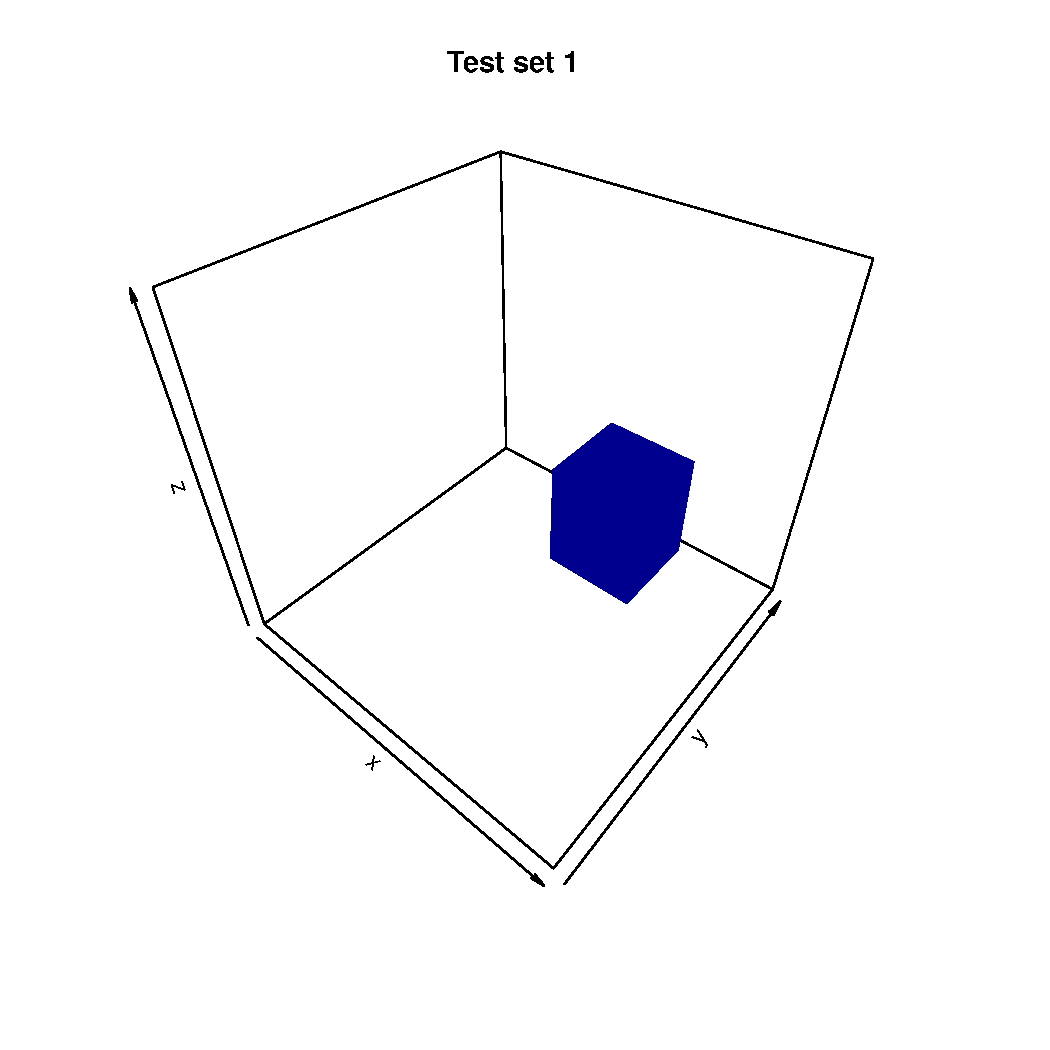
\includegraphics[width=.35\columnwidth]{plots/TS1.pdf} 
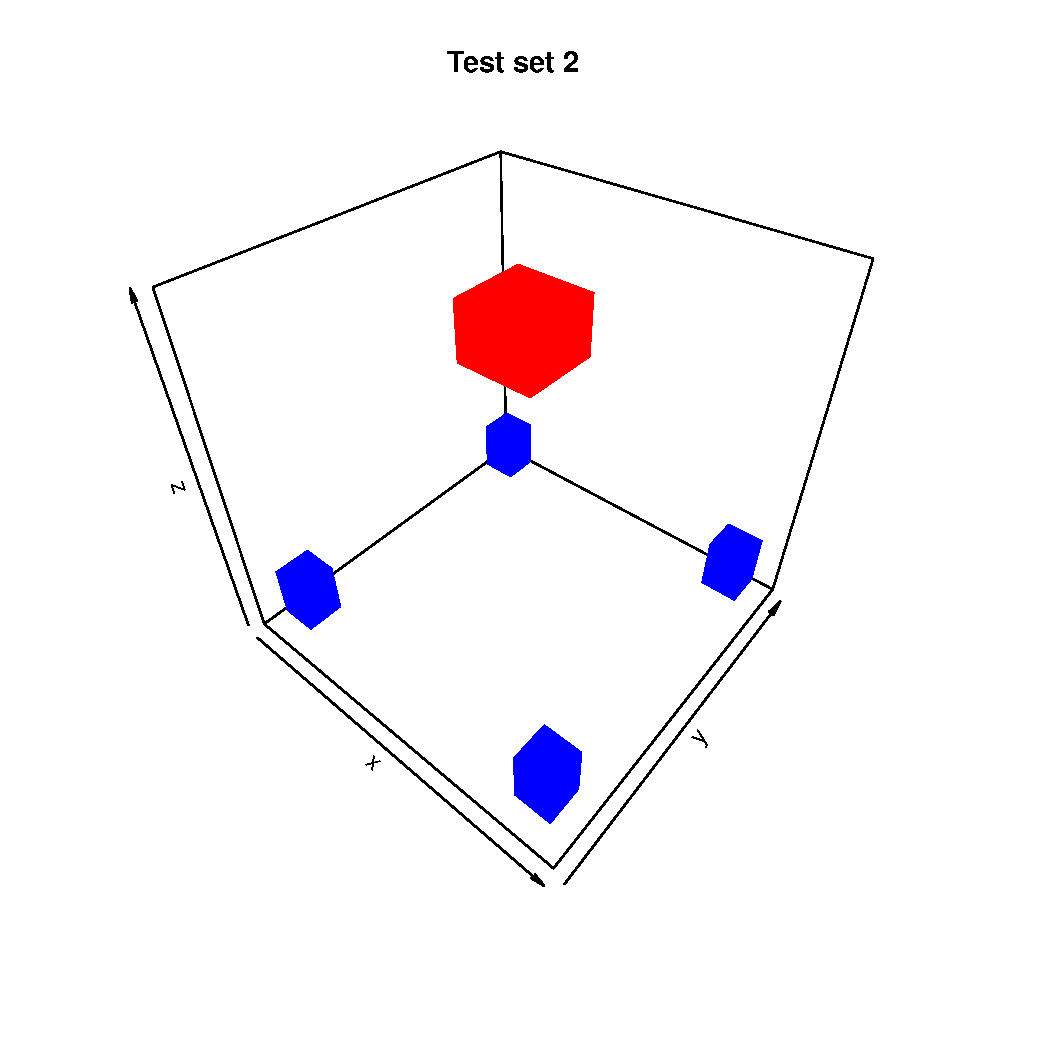
\includegraphics[width=.35\columnwidth]{plots/TS2.pdf} 
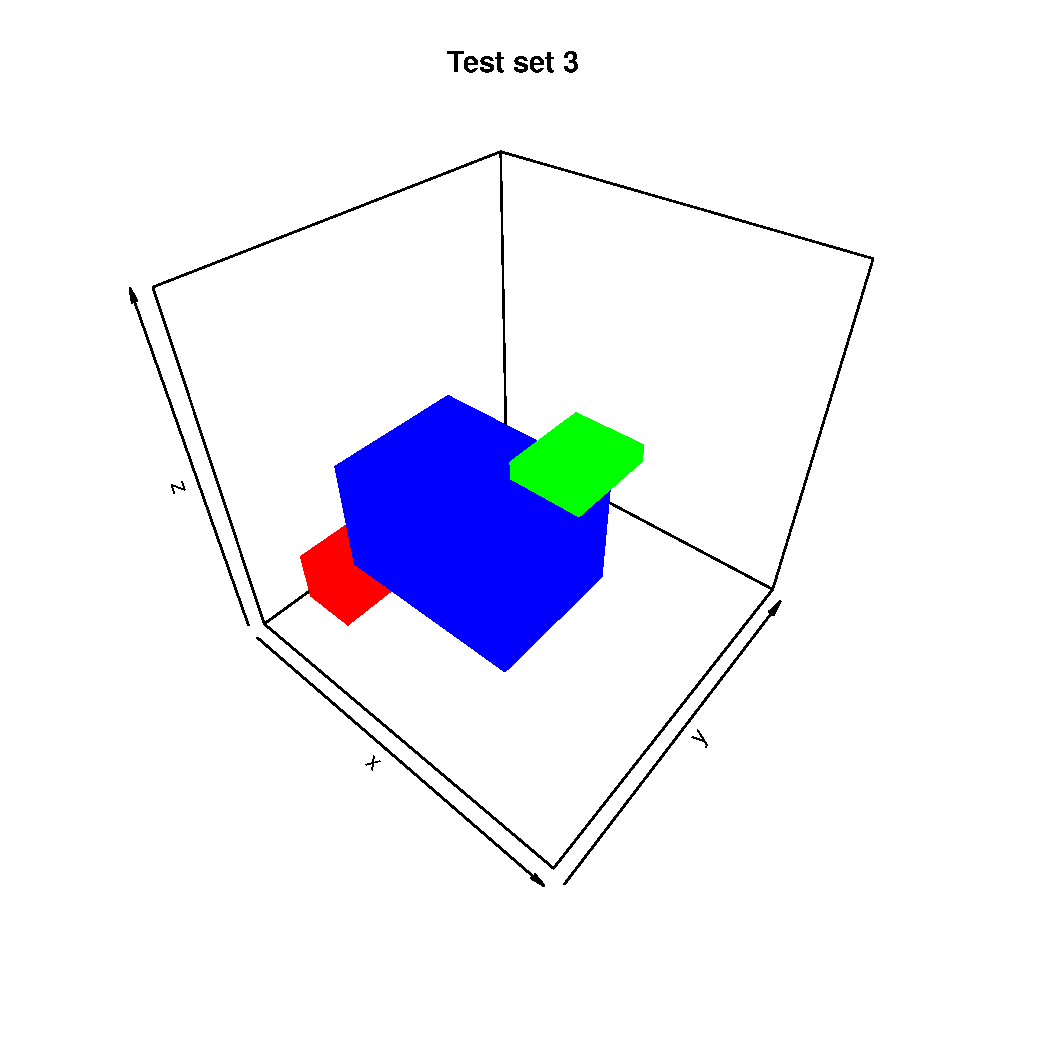
\includegraphics[width=.35\columnwidth]{plots/TS3.pdf} 
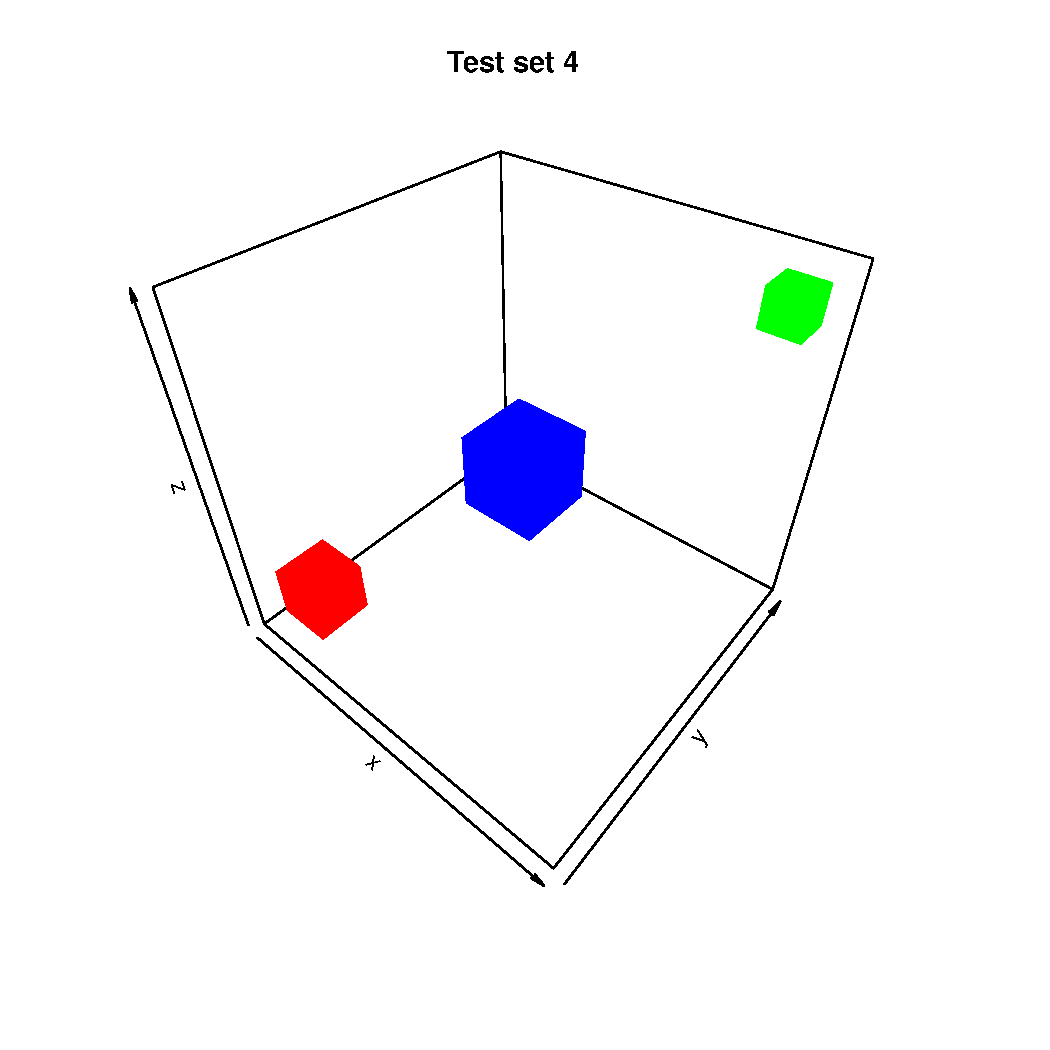
\includegraphics[width=.35\columnwidth]{plots/TS4.pdf} 
\caption{True blocks in test data sets. }
\label{fig: testcases}
\end{figure}

\begin{table}[h]
\centering
\caption{Summary of unit test results in the 3-dimensional space}
\label{table: test3d}
\begin{tabular}{|r|r|r|r|r|r|r|}
\hline
\multicolumn{1}{|c|}{\multirow{2}{*}{\begin{tabular}[c]{@{}c@{}}Dimensionality Selection Policy\\ Density Measure\end{tabular}}} & \multicolumn{3}{c|}{Maximum Density First}                                                  & \multicolumn{3}{c|}{Maximum Cardinality First}                                              \\ \cline{2-7} 
\multicolumn{1}{|c|}{}                                                                                                           & \multicolumn{1}{c|}{Dataset} & \multicolumn{1}{c|}{Precision} & \multicolumn{1}{c|}{Recall} & \multicolumn{1}{c|}{Dataset} & \multicolumn{1}{c|}{Precision} & \multicolumn{1}{c|}{Recall} \\ \hline
\multirow{4}{*}{Arithmatic Average Degree}                                                                                       & Test set 1                   & 1.0                            & 1.0                         & Test set 1                   & 1.0                            & 1.0                         \\ \cline{2-7} 
                                                                                                                                 & Test set 2                   & 1.0                            & 1.0                         & Test set 2                   & 1.0                            & 1.0                         \\ \cline{2-7} 
                                                                                                                                 & Test set 3                   & 1.0                            & 0.978                       & Test set 3                   & 1.0                            & 1.0                         \\ \cline{2-7} 
                                                                                                                                 & Test set 4                   & 1.0                            & 0.922                       & Test set 4                   & 1.0                            & 0.922                       \\ \hline
\multirow{4}{*}{Geometric Average Degree}                                                                                        & Test set 1                   & 1.0                            & 1.0                         & Test set 1                   & 1.0                            & 1.0                         \\ \cline{2-7} 
                                                                                                                                 & Test set 2                   & 1.0                            & 1.0                         & Test set 2                   & 1.0                            & 1.0                         \\ \cline{2-7} 
                                                                                                                                 & Test set 3                   & 1.0                            & 0.978                       & Test set 3                   & 1.0                            & 1.0                         \\ \cline{2-7} 
                                                                                                                                 & Test set 4                   & 1.0                            & 0.922                       & Test set 4                   & 1.0                            & 0.922                       \\ \hline
\multirow{4}{*}{Suspiciousness}                                                                                                  & Test set 1                   & 1.0                            & 1.0                         & Test set 1                   & 1.0                            & 1.0                         \\ \cline{2-7} 
                                                                                                                                 & Test set 2                   & 1.0                            & 1.0                         & Test set 2                   & 1.0                            & 1.0                         \\ \cline{2-7} 
                                                                                                                                 & Test set 3                   & 1.0                            & 1.0                         & Test set 3                   & 1.0                            & 1.0                         \\ \cline{2-7} 
                                                                                                                                 & Test set 4                   & 1.0                            & 0.922                       & Test set 4                   & 1.0                            & 0.922                       \\ \hline
\end{tabular}
\end{table}

\begin{table}[h]
\centering
\caption{Summary of unit tests in the 4-dimensional space}
\label{table: test4d}
\begin{tabular}{|r|r|r|r|r|r|r|}
\hline
\multicolumn{1}{|c|}{\multirow{2}{*}{\begin{tabular}[c]{@{}c@{}}Dimensionality Selection Policy\\ Density Measure\end{tabular}}} & \multicolumn{3}{c|}{Maximum Density First}                                                  & \multicolumn{3}{c|}{Maximum Cardinality First}                                              \\ \cline{2-7} 
\multicolumn{1}{|c|}{}                                                                                                           & \multicolumn{1}{c|}{Dataset} & \multicolumn{1}{c|}{Precision} & \multicolumn{1}{c|}{Recall} & \multicolumn{1}{c|}{Dataset} & \multicolumn{1}{c|}{Precision} & \multicolumn{1}{c|}{Recall} \\ \hline
\multirow{3}{*}{Arithmatic Average Degree}                                                                                       & Test set 1                   & 1.0                            & 1.0                         & Test set 1                   & 1.0                            & 1.0                         \\ \cline{2-7} 
                                                                                                                                 & Test set 2                   & 1.0                            & 0.989                       & Test set 2                   & 1.0                            & 0.989                       \\ \cline{2-7} 
                                                                                                                                 & Test set 3                   & 1.0                            & 0.995                       & Test set 3                   & 1.0                            & 0.995                       \\ \hline
\multirow{3}{*}{Geometric Average Degree}                                                                                        & Test set 1                   & 1.0                            & 1.0                         & Test set 1                   & 1.0                            & 1.0                         \\ \cline{2-7} 
                                                                                                                                 & Test set 2                   & 1.0                            & 0.989                       & Test set 2                   & 1.0                            & 0.989                       \\ \cline{2-7} 
                                                                                                                                 & Test set 3                   & 1.0                            & 0.995                       & Test set 3                   & 1.0                            & 0.995                       \\ \hline
\multirow{3}{*}{Suspiciousness}                                                                                                  & Test set 1                   & 1.0                            & 1.0                         & Test set 1                   & 1.0                            & 1.0                         \\ \cline{2-7} 
                                                                                                                                 & Test set 2                   & 1.0                            & 0.989                       & Test set 2                   & 1.0                            & 0.989                       \\ \cline{2-7} 
                                                                                                                                 & Test set 3                   & 1.0                            & 0.995                       & Test set 3                   & 1.0                            & 0.995                       \\ \hline
\end{tabular}
\end{table}
We summarize the tests based on the above described test sets in Table \ref{table: test3d} and Table \ref{table: test4d}. Given each data set, the output of Dcube algorithm is $k$ blocks. The intersection of the real blocks with positive mass and the $k$ identified blocks can be seen as the true positive results. The entries with positive mass that are not identified by the algorithm can be seen as false negatives, and the entries identified by the algorithm, which have zero mass, are seen as false positives. The precision and recall rates in the following table are calculated using the following formulas.

$$\text{Precision} = \frac{\text{True Positive}}{\text{True Positive + False Positive}}$$
$$\text{Recall} = \frac{\text{True Positive}}{\text{True Positive + False Negative}}$$

As can be seen from Table \ref{table: test3d} and Table \ref{table: test4d}, our current method achieves very high precision and recall score. The majority of blocks are correctly identified, and very little false positive identifications were made.

\subsection{Evaluation}
As is required, we applied the D-cube algorithm on both the DARPA TCP Dump dataset and the Airforce TCP Dump dataset. We used the arithmetic density measure and maximum density policy.

\subsubsection{Top 5 blocks}
We summarize the basic information of the top 5 blocks detected in each dataset in Table \ref{table: k5_2}.

\begin{table}[htbp]
\centering
\caption{Summary of the first 5 blocks on DARPA and Airforce attack dataset}
\label{table: k5_2}
\begin{tabular}{rrrrr}
\hline
Dataset                                                                                    & Order                  & Volume & Mass   & Density  \\ \hline
\multirow{5}{*}{DARPA}                                                                     & \multicolumn{1}{r|}{1} & 94     & 278K   & 16697.28 \\
                                                                                           & \multicolumn{1}{r|}{2} & 2832   & 688K   & 16005.70 \\
                                                                                           & \multicolumn{1}{r|}{3} & 88     & 230K   & 14688.77 \\
                                                                                           & \multicolumn{1}{r|}{4} & 5      & 26K    & 11301.86 \\
                                                                                           & \multicolumn{1}{r|}{5} & 36     & 77K    & 11060.71 \\ \hline
\multirow{5}{*}{Airforce}                                                                  & \multicolumn{1}{r|}{1} & 1      & 1.93M  & 1.93M    \\
                                                                                           & \multicolumn{1}{r|}{2} & 8      & 2.53M  & 1.77M    \\
                                                                                           & \multicolumn{1}{r|}{3} & 131K   & 554K   & 41.7K    \\
                                                                                           & \multicolumn{1}{r|}{4} & 3.71M  & 493K   & 27.2K    \\
                                                                                           & \multicolumn{1}{r|}{5} & 1.4K   & 168.9K & 19K      \\ \hline
\end{tabular}
\end{table}


\subsubsection{ROC curves}

Here, we defined each entry in the dataset labeled as positive as a positive entry. If that entry is identified at a certain stage of the algorithm, then it is regarded as a true positive, otherwise it is regarded as a false negative. Left half of Figure \ref{fig: roc} shows the ROC curve of applying D-cube algorithm on the DARPA TCP Dump dataset with $k = 1, \cdots, 20$. The right half of Figure \ref{fig: roc} similarly shows the ROC curve of D-cube on Airforce TCP Dump dataset. 

\begin{figure}[htbp]
\centering 
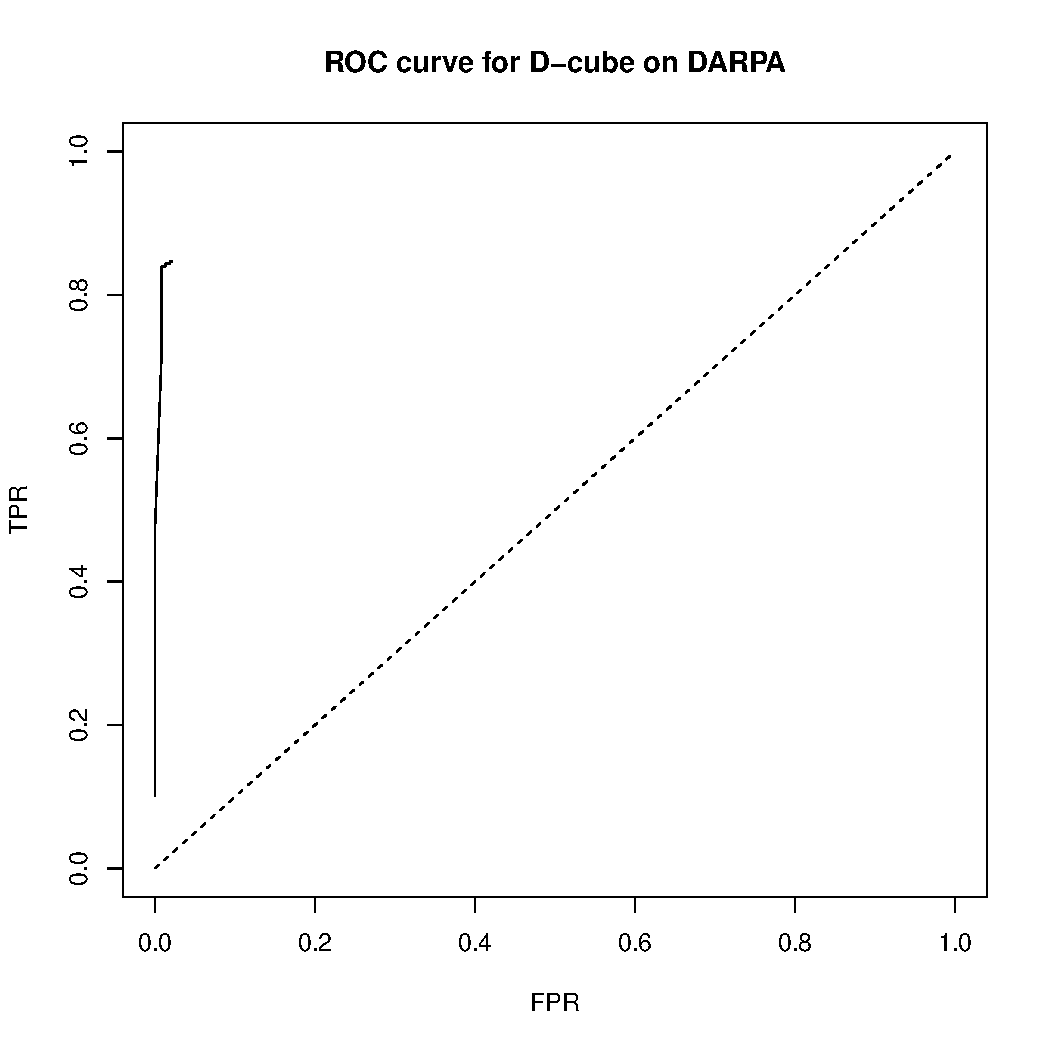
\includegraphics[width=.45\columnwidth]{plots/darpa_ROC.pdf} 
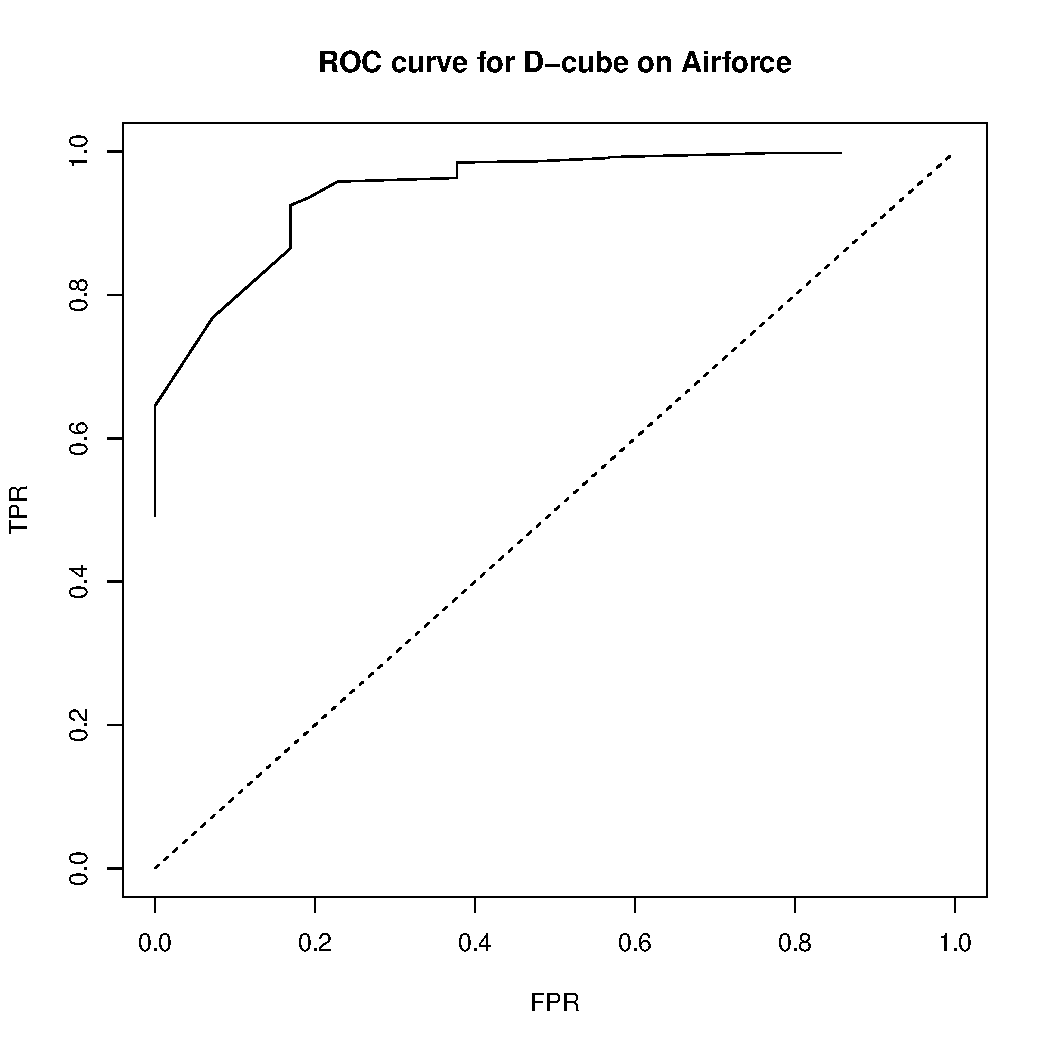
\includegraphics[width=.45\columnwidth]{plots/airforce_ROC.pdf} 
\caption{The ROC curve for $k = 1, \cdots, 20$ by applying the D-cube algorithm on the DARPA TCP Dump dataset (left) and Airforce TCP Dump dataset (right). }
\label{fig: roc}
\end{figure}



%Here, we illustrate the results on DARPA data in Table \ref{table: darpa}, where the timestamps are bucketized by days, and the number of blocks is specified to be $K=1$ due to limited time. We point out that this bucketization by day gives a  very coarse resolution -- all the hours in the entire day are treated as a whole, which will be entirely picked up by a dense block or entirely missed. In addition, when computing the precision and recall rates, the true labels are also bucketized by days: if there is one positive entry in a day, we treat the day as positive as a whole. This is again a rough measurement. Therefore, the current  precision and recall rates are not very high.  More thorough analyses will be conducted in the upcoming experiments (please see the next subsection).

%\begin{table}[]
%\centering
%\caption{Results on the DARPA data set bucketized by day with $K = 1$}
%\label{table: darpa}
%\begin{tabular}{|r|r|r|r|r|}
%\hline
%\multicolumn{1}{|c|}{\multirow{2}{*}{\begin{tabular}[c]{@{}c@{}}Dimensionality Selection Policy\\ Density Measure\end{tabular}}} & \multicolumn{2}{c|}{Density First}                           & \multicolumn{2}{l|}{Cardinality First}                       \\ \cline{2-5} 
%\multicolumn{1}{|c|}{}                                                                                                           & \multicolumn{1}{c|}{Precision} & \multicolumn{1}{c|}{Recall} & \multicolumn{1}{c|}{Precision} & \multicolumn{1}{c|}{Recall} \\ \hline
%Arithmatic Average Degree                                                                                                        & 0.0131                         & 0.0048                      & 0.0175                         & 0.0056                      \\ \hline
%Geometric Average Degree                                                                                                         & 0.0035                         & 0.0023                      & 0.0175                         & 0.0056                      \\ \hline
%Suspiciousness                                                                                                                   & 0.2116                         & 0.3511                      & 0.1458                         & 0.1686                      \\ \hline
%\end{tabular}
%\end{table}

\subsection{Anomaly Detection in Real-world Data}
We also applied our implementation on the other three real-world datasets using maximum density policy for dimension selection. We used arithmetic density measure for Yelp and Amazon dataset, and geometric density measure for Wikipedia dataset. Table \ref{table: k5_3} summarizes the information for the first five blocks identified in each dataset.

\begin{table}[htbp]
\centering
\caption{Summary of the first 5 blocks on Yelp, Amazon, and Wiki dataset}
\label{table: k5_3}
\begin{tabular}{rrrrr}
\hline
Dataset                                                                                    & Order                  & Volume & Mass   & Density  \\ \hline
\multirow{5}{*}{Yelp}                                                                      & \multicolumn{1}{r|}{1} & 3600   & 3600   & 118.03   \\
                                                                                           & \multicolumn{1}{r|}{2} & 3025   & 3025   & 108.04   \\
                                                                                           & \multicolumn{1}{r|}{3} & 2500   & 2500   & 98.04    \\
                                                                                           & \multicolumn{1}{r|}{4} & 2025   & 2025   & 88.04    \\
                                                                                           & \multicolumn{1}{r|}{5} & 336.7B & 268K   & 84.83    \\ \hline
\multirow{5}{*}{Amazon}                                                                    & \multicolumn{1}{r|}{1} & 3600   & 3600   & 118.03   \\
                                                                                           & \multicolumn{1}{r|}{2} & 135K   & 7550   & 99.02    \\
                                                                                           & \multicolumn{1}{r|}{3} & 1600   & 1600   & 78.05    \\
                                                                                           & \multicolumn{1}{r|}{4} & 1225   & 1225   & 68.06    \\
                                                                                           & \multicolumn{1}{r|}{5} & 30B    & 77.7K  & 50.34    \\ \hline
\multirow{5}{*}{\begin{tabular}[c]{@{}r@{}}Wikipedia\\ (Geometric\\ Density)\end{tabular}} & \multicolumn{1}{r|}{1} & 32     & 7865   & 2477.32  \\
                                                                                           & \multicolumn{1}{r|}{2} & 6696   & 16508  & 875.84   \\
                                                                                           & \multicolumn{1}{r|}{3} & 5      & 557    & 325.74   \\
                                                                                           & \multicolumn{1}{r|}{4} & 10     & 110    & 51.06    \\
                                                                                           & \multicolumn{1}{r|}{5} & 1974   & 6491   & 517.44   \\ \hline
\end{tabular}
\end{table}






    
% \input{upcoming-expr}

\section{Concolusion}
    \label{sec:concolusion}
    %!TEX root = final_report.tex

In this project, we provide an implementation of the D-Cube algorithm for dense block detection using PostgreSQL. Our implementation stores all information on disk using SQL relations, and is able to handle large real-world dataset even when the data and metadata cannot fit in memory.  We compare different optimization methods, and find that for the D-Cube algorithm, iteratively deleting the required entries from relations is more efficient than adding an extra column to mark the deletion. We also find that creating index for relations that are repeatedly queried can significantly reduce the computation time. 


\section{Graded Phase 1 \& 2 }

Please see below for a screenshot in Blackboard. We got 100/100 in both phase 1 and phase 2.

\begin{figure}[h]
\centering 

\includegraphics[width=.75\columnwidth]{plots/phase1.png} 
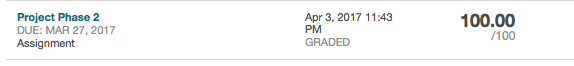
\includegraphics[width=.75\columnwidth]{plots/phase2.png} 
\end{figure}

\bibliography{database}
\bibliographystyle{plain}


\end{document}
